% ex: ts=2 sw=2 sts=2 et filetype=tex
% SPDX-License-Identifier: CC-BY-SA-4.0

\documentclass[10pt,addpoints]{exam}

\usepackage[utf8]{inputenc}
\usepackage[T1]{fontenc}
%\usepackage[spanish]{babel}
\usepackage[letterpaper]{geometry}
\usepackage{graphicx}
\usepackage{pgfplots}
\usepackage{multicol}
\setlength{\columnsep}{2cm}

\pagestyle{headandfoot}
\headrule
\header{Matemáticas aplicadas}{Intersemestrales}{CBTIS 246}
\footer{}{Página \thepage\ de \numpages}{}

\pointpoints{punto}{puntos}
\renewcommand{\solutiontitle}{\textbf{Solución: }}

%\printanswers

\begin{document}

Nombre:\enspace\hrulefill

\vspace{5mm}

Grupo:\enspace\hrulefill
\enspace{}Grado:\enspace\hrulefill
\enspace{}Fecha:\enspace\hrulefill

\begin{questions}

\begin{EnvFullwidth}
  \sffamily\textbf{Investiga y respesponde las siguientes pregutnas.}
\end{EnvFullwidth}

% ex: ts=2 sw=2 sts=2 et filetype=tex
% SPDX-License-Identifier: CC-BY-SA-4.0

\question  Es la medida de la superficie que abarca una figura y se mide en
           $cm^2$, $m^2$, etc.

  \begin{oneparchoices}
    \CorrectChoice Área
    \choice Perimetro
    \choice Volumen
  \end{oneparchoices}

% ex: ts=2 sw=2 sts=2 et filetype=tex
% SPDX-License-Identifier: CC-BY-SA-4.0

\question ¿Para qué sirve una succesión?
  \begin{solution}[2cm]
    Sirve para modelar patrones, predecir el comportamiento futuro de
    fenómenos basados en secuencias.
  \end{solution}

% ex: ts=2 sw=2 sts=2 et filetype=tex
% SPDX-License-Identifier: CC-BY-SA-4.0

\question ¿Qué tipos de sucesiónes hay?:
  \begin{solution}[2cm]
    Se clasifican en aritméticas, gemétricas, alfanuméricas y simbólicas
  \end{solution}

% ex: ts=2 sw=2 sts=2 et filetype=tex
% SPDX-License-Identifier: CC-BY-SA-4.0

\question La \fillin[P. Directa] ocurre cuando dos cantidades aumentan ó
          disminuyen al mismo ritmo. Es decir, si una variable aumenta ó
          disminuye la otra tamién en la misma proporción 


% ex: ts=2 sw=2 sts=2 et filetype=tex
% SPDX-License-Identifier: CC-BY-SA-4.0

\question Dos magnitudes son inversamente proporcionales cuando al aumentar
          una, la otra disminuye en la misma proporción. A esto se le llama:
          \fillin[Proporcional inversa]

% ex: ts=2 sw=2 sts=2 et filetype=tex
% SPDX-License-Identifier: CC-BY-SA-4.0

\question Define que es la suceción alfanumérica/simbólica:
  \begin{solution}[2cm]
    La alfanumérica consta de números y letras, y la simbólica utiliza
    dibujos.
  \end{solution}


\newpage

% ex: ts=2 sw=2 sts=2 et filetype=tex
% SPDX-License-Identifier: CC-BY-SA-4.0

\question Escribe un ejemplo de cada una de las sucesiones definidas
          anteriormente:
  \begin{solution}[4cm]
    \textbf{Aritméticas:} 2,5,8,11,14,17,20 (usando sumas, aqui suma 3) \\
    \textbf{Geométricas:}  2,6,18,54,162 (usando una multiplicación por 3) \\
    \textbf{Alfanuméricas:} 2a,6c,18e,54f,162,h (usando letras y números) \\
    \textbf{Simbólicas:} (usando dibujos)
  \vspace{1cm}
  \end{solution}

% ex: ts=2 sw=2 sts=2 et filetype=tex
% SPDX-License-Identifier: CC-BY-SA-4.0

\question ¿Qué es rotación, traslación y percepción espacial?:
  \begin{solution}[4cm]
    \textbf{Rotación:} Cuando un cuerpo gira alrededor de un eje. \\
    \textbf{Traslación:} Cuando un cuerpo cambia de posición inicial a una
                         final. \\
    \textbf{Percepción espacial:} Habilidad de comprender la posición de los
                                  objetos en el espacio.
  \vspace{1cm}
  \end{solution}


%%%%%%%%%%%%%%%%%%%%%%%%%%%%%%%%%%%%%%%%%%%

\begin{EnvFullwidth}
  \sffamily\textbf{Une con una línea la respuesta que corresponde.}
\end{EnvFullwidth}

% ex: ts=2 sw=2 sts=2 et filetype=tex
% SPDX-License-Identifier: CC-BY-SA-4.0

\begin{multicols}{2}
  \question Son secuencias de números reales ordenados y deben tener un
            primer termino.

  \question Son las sucesiones donde el término siguiente se obtiene
            multiplicando al anterior por una cantidad constante llamada
            razón.

  \question Es la sucesión que consta de números y letras.

\columnbreak

  \begin{enumerate}
    \item[a)] Suseciones alfanumericas
    \vspace{\baselineskip}
    \item[b)] Sucesiones
    \vspace{\baselineskip}
    \item[c)] Sucesiones geométricas
    \vspace{\baselineskip}
    \item[d)] Secuencias numéricas
  \end{enumerate}
\end{multicols}


\begin{EnvFullwidth}
  \sffamily\textbf{Lee con atención cada pregunta y responde en
  el espacio indicado. }
\end{EnvFullwidth}

% ex: ts=2 sw=2 sts=2 et filetype=tex
% SPDX-License-Identifier: CC-BY-SA-4.0

\question De la siguiente suceción
\[
2,7,12,17
\]
\begin{parts}
  \part Escribe los 4 números siguientes: \fillin[22][1.5cm],
  \fillin[27][1.5cm], \fillin[32][1.5cm], \fillin[37][1.5cm].

  \part ¿Cuál es la diferencia? \fillin[5]

  \part Crea un modelo matemático que la represente: \fillin[2 + 5(n)]

  \part Calcula los términos de $n_3=$\fillin[17][1.5cm],
  $n_7=$\fillin[37][1.5cm], $n_9=$\fillin[47][1.5cm],
  $n_{25}=$\fillin[157][1.5cm].
\end{parts}

\vspace{\baselineskip}

% ex: ts=2 sw=2 sts=2 et filetype=tex
% SPDX-License-Identifier: CC-BY-SA-4.0

\question ¿Cuál es el alor de f(2) si $f(x) = 3x + 1$?

  \begin{oneparchoices}
    \choice 4
    \choice 6
    \CorrectChoice  7
  \end{oneparchoices}

\vspace{\baselineskip}

% ex: ts=2 sw=2 sts=2 et filetype=tex
% SPDX-License-Identifier: CC-BY-SA-4.0

\question \[ \frac{9}{7} \times \frac{3}{2} = \frac{\hspace{2cm}}{\hspace{2cm}} 
             \hspace{2cm}
             \frac{7}{3} \times \frac{4}{6} = \frac{\hspace{2cm}}{\hspace{2cm}}
          \]


\vspace{\baselineskip}

% ex: ts=2 sw=2 sts=2 et filetype=tex
% SPDX-License-Identifier: CC-BY-SA-4.0

\question ¿Cómo se escribe en notación cientifica el siguiente valor
  $0.0000982$?

  \begin{oneparchoices}
    \choice $9.82\times10^{-2}$
    \choice $9.82\times10^{-0}$
    \choice $9.82\times10^{3}$
    \CorrectChoice $9.82\times10^{-5}$
  \end{oneparchoices}
  \answerline[D]


%%%%%%%%%%%%%%%%%%%%%%%%%%%%%%%%%%%%%%%%%%%

\begin{EnvFullwidth}
  \sffamily\textbf{Selecciona la respuesta correcta. }
\end{EnvFullwidth}

\vspace{\baselineskip}
% ex: ts=2 sw=2 sts=2 et filetype=tex
% SPDX-License-Identifier: CC-BY-SA-4.0

\question Es la capacidad física para realizar un trabajo o un movimento.

  \begin{oneparchoices}
    \choice Rapidez
    \choice Aceleración
    \choice Rozamiento
    \CorrectChoice Fuerza
  \end{oneparchoices}
  \answerline[D]

\vspace{\baselineskip}
% ex: ts=2 sw=2 sts=2 et filetype=tex
% SPDX-License-Identifier: CC-BY-SA-4.0

\question Es el cociente entre la frecuencia absoluta de un determinado
valor y el número total de datos

  \begin{oneparchoices}
    \choice Frecuencia acumulada
    \CorrectChoice Frecuencia relativa
    \choice Frecuencia absoluta
  \end{oneparchoices}

% ex: ts=2 sw=2 sts=2 et filetype=tex
% SPDX-License-Identifier: CC-BY-SA-4.0

\question La formula de la ley de la dinamica es:

  \begin{oneparchoices}
    \choice $F=m \cdot v$
    \CorrectChoice $F=m \cdot a$
    \choice $\Sigma F = 0 \Leftrightarrow \frac{dv}{dt} = 0$
    \choice $F_{1 \rightarrow 2} = F_{2 \rightarrow 1}$
  \end{oneparchoices}
  \answerline[B]

% ex: ts=2 sw=2 sts=2 et filetype=tex
% SPDX-License-Identifier: CC-BY-SA-4.0

\question $81a^4b^6 - 25y^8$



%%%%%%%%%%%%%%%%%%%%%%%%%%%%%%%%%%%%%%%%%%%

\newpage

% ex: ts=2 sw=2 sts=2 et filetype=tex
% SPDX-License-Identifier: CC-BY-SA-4.0

\question Usa la siguiente cuadricula para resolver los siguientes incisos:

  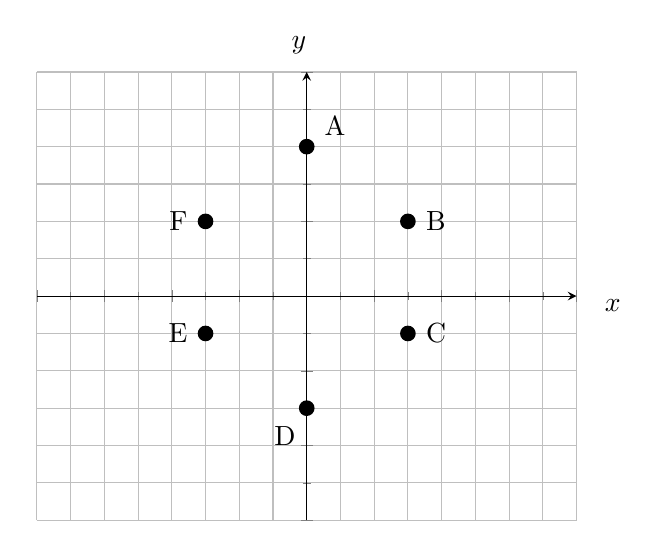
\begin{tikzpicture}
    \begin{axis}[grid=both,ymin=-6,ymax=6,xmax=8,xmin=-8,xticklabel=\empty,yticklabel=\empty,
               minor tick num=1,axis lines = middle,xlabel=$x$,ylabel=$y$,
               label style = {at={(ticklabel cs:1.1)}}]
      \node[label={10:{A}},circle,fill,inner sep=2pt] at (axis cs:0,4) {};
      \node[label={0:{B}},circle,fill,inner sep=2pt] at (axis cs:3,2) {};
      \node[label={0:{C}},circle,fill,inner sep=2pt] at (axis cs:3,-1) {};
      \node[label={260:{D}},circle,fill,inner sep=2pt] at (axis cs:0,-3) {};
      \node[label={180:{E}},circle,fill,inner sep=2pt] at (axis cs:-3,-1) {};
      \node[label={180:{F}},circle,fill,inner sep=2pt] at (axis cs:-3,2) {};
    \end{axis}
  \end{tikzpicture}

  \begin{parts}
    \part Encuantra las coordenadas de los vértices en el polígono. \\
    A(\fillin\ ,\fillin\ ) \enspace B(\fillin\ ,\fillin\ ) \\
    C(\fillin\ ,\fillin\ ) \enspace D(\fillin\ ,\fillin\ ) \\
    E(\fillin\ ,\fillin\ ) \enspace F(\fillin\ ,\fillin\ ) \\
    \part Determina el cuadrante en el que se ubica los puntos: \\
    El punto B esta en el cuadrante:\fillin \\
    El punto C esta en el cuadrante:\fillin \\
    El punto E esta en el cuadrante:\fillin \\
    El punto F esta en el cuadrante:\fillin \\
    \part Sacar la distancia entre los puntos: \\
    AB \fillin \enspace BC \fillin \enspace CD \fillin \\
    DE \fillin \enspace EF \fillin \enspace FA \fillin \\
    \part Calcula el perímetro de la figura resultante.
  \end{parts}


\newpage

% ex: ts=2 sw=2 sts=2 et filetype=tex
% SPDX-License-Identifier: CC-BY-SA-4.0

\question Se realiza una fuerza \fillin \enspace, cuando un cuerpo empuja
          a otro.

  \begin{oneparchoices}
    \choice De empuje
    \choice De velocidad
    \choice De fricción
    \CorrectChoice De contacto
  \end{oneparchoices}
  \answerline[D]

% ex: ts=2 sw=2 sts=2 et filetype=tex
% SPDX-License-Identifier: CC-BY-SA-4.0

\question Resuelve las siguientes ecuaciones y compruebalos sustituyendo el
          valor de $x$

  \begin{parts}
    \part $6x+4 = 3x+10$ \\
    \\
    \\
    \\
    \part $6x+3 = 2x+11$ \\
    \\
    \\
    \\
    \part $2x+5 = x-3$
  \end{parts}


\end{questions}

\end{document}
